\section{Branches, Connectors, and Nodes}\label{branches-connectors-and-nodes}

In EnergyPlus, the HVAC system and plant form a network (technically, a graph). The individual pieces of equipment -- the fans, coils, chillers, etc. -- are connected together by air ducts and fluid pipes. In EnergyPlus nomenclature, the air and fluid circuits are called loops. Specifying how an individual system and plant are connected is done in the EnergyPlus input (IDF) file. The overall structure of the network is defined with Branch and Connector objects. The detail is filled with components and their inlet and outlet nodes. A Branch consists of one or more components arranged sequentially along a pipe or duct. A Connector specifies how three or more branches are connected through a Splitter or Mixer. Nodes connect components along a branch: the outlet node of one component is the inlet node of the next downstream component. The nodes represent conditions at a point on a loop. Each component has one or more inlet and outlet nodes, depending on how many loops it interacts with. A fan, for instance, has one inlet node and one outlet node, since it interacts with a single air loop. A water coil will have 2 inlet and 2 outlet nodes, since it interacts with an air and a fluid loop. Figure~\ref{fig:hvac-input-diagram} shows a diagram of an EnergyPlus HVAC input.

\begin{figure}[hbtp] % fig 1
\centering
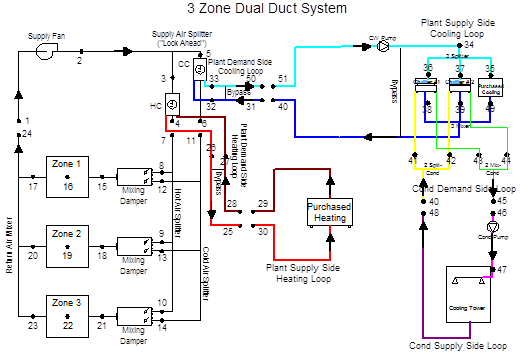
\includegraphics[width=0.9\textwidth, height=0.9\textheight, keepaspectratio=true]{media/image002.png}
\caption{  HVAC Input Diagram \protect \label{fig:hvac-input-diagram}}
\end{figure}

As an illustration of how such a network is built up on the IDF, here is the section of the IDF that describes the supply fan, splitter, and heating and cooling coil section of the dual duct air system.

\textbf{BranchList,}

~~~ Dual Duct Air Loop Branches,~ !- Name

~~~ Air Loop Main Branch,~~~ !- Branch 1 Name

~~~ Heating Coil Air Sys Branch,~ !- Branch 2 Name

~~~ Cooling Coil Air Sys Branch;~ !- Branch 3 Name

\textbf{ConnectorList,}

~~~ Dual Duct Connectors,~~~ !- Name

~~~ Connector:Splitter,~~~~~ !- Connector 1 Object Type

~~~ DualDuctAirSplitter;~~~~ !- Connector 1 Name

\textbf{NodeList,}

~~~ Zone Equipment Inlet Node List,~ !- Name

~~~ Main Hot Air Inlet,~~~~~ !- Node 1 Name

~~~ Main Cold Air Inlet;~~~~ !- Node 2 Name

\textbf{NodeList,}

~~~ Air Loop Outlet Node List,~ !- Name

~~~ Heating Coil Outlet Node,!- Node 1 Name

~~~ Cooling Coil Outlet Node;!- Node 2 Name

\textbf{Branch,}

~~~ Air Loop Main Branch,~~~ !- Name

~~~ ,~~~~~~~~~~~~~~~ !- Pressure Drop Curve Name

~~~ Fan:ConstantVolume,~~~~~ !- Component 1 Object Type

~~~ Supply Fan 1,~~~~~~~~~~~ !- Component 1 Name

~~~ Supply Fan Inlet Node,~~ !- Component 1 Inlet Node Name

~~~ Supply Fan Outlet Node;~ !- Component 1 Outlet Node Name


\textbf{Branch,}

~~~ Heating Coil Air Sys Branch,~ !- Name

~~~ ,~~~~~~~~~~~~~~~ !- Pressure Drop Curve Name

~~~ Coil:Heating:Water,~~~~~ !- Component 1 Object Type

~~~ Main Heating Coil,~~~~~~ !- Component 1 Name

~~~ Heating Coil Inlet Node, !- Component 1 Inlet Node Name

~~~ Heating Coil Outlet Node;!- Component 1 Outlet Node Name

\textbf{Branch,}

~~~ Cooling Coil Air Sys Branch,~ !- Name

~~~ ,~~~~~~~~~~~~~~~ !- Pressure Drop Curve Name

~~~ Coil:Cooling:Water,~~~~~ !- Component 1 Object Type

~~~ Simple Cooling Coil,~~~~ !- Component 1 Name

~~~ Cooling Coil Inlet Node, !- Component 1 Inlet Node Name

~~~ Cooling Coil Outlet Node;!- Component 1 Outlet Node Name

\textbf{Connector:Splitter,}

~~~ DualDuctAirSplitter,~~~~ !- Name

~~~ Air Loop Main Branch,~~~ !- Inlet Branch Name

~~~ Heating Coil Air Sys Branch,~ !- Outlet Branch 1 Name

~~~ Cooling Coil Air Sys Branch;~ !- Outlet Branch 2 Name

\textbf{Fan:ConstantVolume,}

~~~ Supply Fan 1,~~~~~~~~~~~ !- Name

~~~ FanAndCoilAvailSched,~~~ !- Availability Schedule Name

~~~ 0.7,~~~~~~~~~~~~~~~~~~~~ !- Fan Efficiency

~~~ 600.0,~~~~~~~~~~~~~~~~~~ !- Pressure Rise \{Pa\}

~~~ autosize,~~~~~~~~~~~~~~~ !- Maximum Flow Rate \{m3/s\}

~~~ 0.9,~~~~~~~~~~~~~~~~~~~~ !- Motor Efficiency

~~~ 1.0,~~~~~~~~~~~~~~~~~~~~ !- Motor In Airstream Fraction

~~~ Supply Fan Inlet Node,~~ !- Fan Inlet Node Name

~~~ Supply Fan Outlet Node;~ !- Fan Outlet Node Name

\textbf{Coil:Cooling:Water,}

~~~ Simple Cooling Coil,~~~~ !- Name

~~~ CoolingCoilAvailSched,~~ !- Availability Schedule Name

~~~ autosize,~~~~~~~~~~~~~~~ !- Design Water Flow Rate \{m3/s\}

~~~ autosize,~~~~~~~~~~~~~~~ !- Design Air Flow Rate \{m3/s\}

~~~ autosize,~~~~~~~~ !- Design Inlet Water Temperature \{C\}

~~~ autosize,~~~~~~~~ !- Design Inlet Air Temperature \{C\}

~~~ autosize,~~~~~~~~ !- Design Outlet Air Temperature \{C\}

~~~ autosize,~~~~ !- Design Inlet Air Humidity Ratio \{kg-H2O/kg-air\}

~~~ autosize,~~~~ !- Design Outlet Air Humidity Ratio \{kg-H2O/kg-air\}

~~~ Cooling Coil Water Inlet Node,~ !- Water Inlet Node Name

~~~ Cooling Coil Water Outlet Node,~ !- Water Outlet Node Name

~~~ Cooling Coil Inlet Node, !- Air Inlet Node Name

~~~ Cooling Coil Outlet Node,!- Air Outlet Node Name

~~~ SimpleAnalysis,~~~~~~~~~ !- Type of Analysis

~~~ CrossFlow;~~~~~~~~~~~~~~ !- Heat Exchanger Configuration

\textbf{AirLoopHVAC:ZoneSplitter,}

~~~ ZoneColdAirSupplySplitter,~ !- Name

~~~ Main Cold Air Inlet,~~~~ !- Inlet Node Name

~~~ Zone 1 Dual Duct Cold Inlet,~ !- Outlet 1 Node Name

~~~ Zone 2 Dual Duct Cold Inlet,~ !- Outlet 2 Node Name

~~~ Zone 3 Dual Duct Cold Inlet;~ !- Outlet 3 Node Name

\textbf{AirLoopHVAC:ZoneSplitter,}

~~~ ZoneHotAirSupplySplitter,!- Name

~~~ Main Hot Air Inlet,~~~~~ !- Inlet Node Name

~~~ Zone 1 Dual Duct Hot Inlet,~ !- Outlet 1 Node Name

~~~ Zone 2 Dual Duct Hot Inlet,~ !- Outlet 2 Node Name

~~~ Zone 3 Dual Duct Hot Inlet;~ !- Outlet 3 Node Name

\textbf{AirLoopHVAC:ZoneMixer,}

~~~ ZoneReturnAirMixer,~~~~~ !- Name

~~~ Return Air Mixer Outlet, !- Outlet Node Name

~~~ Zone 1 Outlet Node,~~~~~ !- Inlet 1 Node Name

~~~ Zone 2 Outlet Node,~~~~~ !- Inlet 2 Node Name

~~~ Zone 3 Outlet Node;~~~~~ !- Inlet 3 Node Name

\textbf{Coil:Heating:Water,}

~~~ Main Heating Coil,~~~~~~ !- Name

~~~ FanAndCoilAvailSched,~~~ !- Availability Schedule Name

~~~ autosize,~~~~~~~~~~~~~~~ !- U-Factor Times Area Value \{W/K\}

~~~ autosize,~~~~~~~~~~~~~~~ !- Maximum Water Flow Rate \{m3/s\}

~~~ Heating Coil Water Inlet,!- Water Inlet Node Name

~~~ Heating Coil Water Outlet,~ !- Water Outlet Node Name

~~~ Heating Coil Inlet Node, !- Air Inlet Node Name

~~~ Heating Coil Outlet Node,!- Air Outlet Node Name

~~~ UFactorTimesAreaAndDesignWaterFlowRate,~ !- Performance Input Method

~~~ autosize,~~~~~~~~~~~~~~~ !- Nominal Capacity \{W\}

~~~ 82.2,~~~~~~~~~~~~~~~~~~~ !- Design Inlet Water Temperature \{C\}

~~~ 16.6,~~~~~~~~~~~~~~~~~~~ !- Design Inlet Air Temperature \{C\}

~~~ 71.1,~~~~~~~~~~~~~~~~~~~ !- Design Outlet Water Temperature \{C\}

~~~ 32.2;~~~~~~~~~~~~~~~~~~~ !- Design Outlet Air Temperature \{C\}

\textbf{Controller:WaterCoil,}

~~~ Main Cooling Coil Controller,~ !- Name

~~~ Temperature,~~~~~~~~~~~~ !- Control Variable

~~~ Reverse,~~~~~~~~~~~~~~~~ !- Action

~~~ FLOW,~~~~~~~~~~~~~~~~~~~ !- Actuator Variable

~~~ Cooling Coil Outlet Node,!- Sensor Node Name

~~~ Cooling Coil Water Inlet Node, ~!- Actuator Node Name

~~~ 0.001,~~~~~~~~~~~~ !- Controller Convergence Tolerance \{deltaC\}

~~~ autosize,~~~~~~~~~~~~~~~ !- Maximum Actuated Flow \{m3/s\}

~~~ 0.0;~~~~~~~~~~~~~~~~~~~~ !- Minimum Actuated Flow \{m3/s\}

\textbf{Controller:WaterCoil,}

~~~ Main Heating Coil Controller,~ !- Name

~~~ Temperature,~~~~~~~~~~~~ !- Control Variable

~~~ Normal,~~~~~~~~~~~~~~~~~ !- Action

~~~ FLOW,~~~~~~~~~~~~~~~~~~~ !- Actuator Variable

~~~ Heating Coil Outlet Node,!- Sensor Node Name

~~~ Heating Coil Water Inlet,!- Actuator Node Name

~~~ 0.01,~~~~~~~~~~~~~ !- Controller Convergence Tolerance \{deltaC\}

~~~ autosize,~~~~~~~~~~~~~~~ !- Maximum Actuated Flow \{m3/s\}

~~~ 0.0;~~~~~~~~~~~~~~~~~~~~ !- Minimum Actuated Flow \{m3/s\}

Obviously, the creation of such a system/plant network description is best handled by a graphical user interface (GUI). However, for testing purposes a developer may have to create the input for a component by hand and insert it into an existing IDF. Then the developer must be careful to choose unique names for the branches and nodes and make sure the entire network makes physical sense.
